%%%% Proceedings format for most of ACM conferences (with the exceptions listed below) and all ICPS volumes.
\documentclass[sigconf]{acmart}
\usepackage{graphicx}
\usepackage{paralist}
\usepackage{booktabs}
\usepackage{tabularx}
\usepackage{url}
\usepackage[hyphenbreaks]{breakurl}

\def\UrlBreaks{\do\/\do-}

%%%% As of March 2017, [siggraph] is no longer used. Please use sigconf (above) for SIGGRAPH conferences.

%%%% Proceedings format for SIGPLAN conferences 
% \documentclass[sigplan, anonymous, review]{acmart}

%%%% Proceedings format for SIGCHI conferences
% \documentclass[sigchi, review]{acmart}

%%%% To use the SIGCHI extended abstract template, please visit
% https://www.overleaf.com/read/zzzfqvkmrfzn

\usepackage{booktabs} % For formal tables


% Copyright
%\setcopyright{none}
%\setcopyright{acmcopyright}
\setcopyright{acmlicensed}
%\setcopyright{rightsretained}
%\setcopyright{usgov}
%\setcopyright{usgovmixed}
%\setcopyright{cagov}
%\setcopyright{cagovmixed}

\copyrightyear{2018}
\acmYear{2018}
\setcopyright{acmlicensed}
\acmConference[SSEI2018]{Social Sensing and Enterprise Intelligence}{Apr. 23, 2018}{Lyon, France}
% ACM had "Computing" instead of Computer, please update
%\acmBooktitle{}
% \acmPrice{15.00}
% \acmDOI{10.1145/}
% \acmISBN{}
% This slight change to the code may also save 1 or 2 lines of space.

% removes the headers from each page per the preparation instructions, as these are not needed and will be updated with the chairs' actual session names during the pagination/indexing process:
\fancyhead{}

\begin{document}
\title[Evaluation of Performance and Competition of Customer Services on
  Twitter]{Evaluation of Performance and Competition of Customer Services on
  Twitter: A UK Telecoms Case Study}
%\titlenote{}
%\subtitle{Extended Abstract}
%\subtitlenote{}

\author{Nabeel Albishry}
%\orcid{}
\affiliation{%
  \institution{University of Bristol}
  \streetaddress{}
  \city{} 
  \country{United Kingdom}
}
\email{n.albishry@bristol.ac.uk}

\author{Tom Crick}
\orcid{0000-0001-5196-9389}
\affiliation{%
  \institution{Swansea University}
  \streetaddress{}
  \city{} 
  \country{United Kingdom}
}
\email{tcrick@bcs.org.uk}

\author{Theo Tryfonas}

\affiliation{%
  \institution{University of Bristol}
  \streetaddress{}
  \city{} 
  \country{United Kingdom}
}
\email{theo.tryfonas@bristol.ac.uk}

\author{Tesleem Fagade}

\affiliation{%
  \institution{University of Bristol}
  \streetaddress{}
  \city{} 
  \country{United Kingdom}
}
\email{tesleem.fagade@bristol.ac.uk}


 
% The default list of authors is too long for headers}
\renewcommand{\shortauthors}{Albishry, Crick, Tryfonas, and Fagade}


\begin{abstract}
With the increasing number of users on a variety of social media
platforms, customer service-focused organisations are recognising the
importance of social network engagement with their customers. In turn,
consumers judge organisations on the quality of customer service and
degree of responsiveness to queries. This paper presents an extensible
framework for evaluating direct engagements of customer services with
customers. It also measures indirect engagement with business rivals,
competition and their patterns and severity. By using graphs analysis
of Twitter interactions, our approach was used to provide analytical
measures and visual representations for seven UK telecoms
companies. With a dataset consisting of 15,000 tweets and 3,500 user
profiles, the results show that business providers have indirect
engagements with their rivals, and customers are the triggering factor
of those competition.
\end{abstract}

\keywords{TBC}

\maketitle

\section{Introduction}\label{intro}

The microblogging site Twitter has become one of the main social
network platforms, providing a rich corpus of big social data to study
a range of interesting socio-cultural themes, from life event
detection~\cite{blamey-et-al-2013} and identifying language
communities~\cite{albishry-et-al:iccci2017}, through to providing
deeper insight into personality and
behaviour~\cite{mostafa-et-al-ai2016}. Twitter is increasingly being
used by organisation to communicate with customers, as it is fast and
convenient medium of engagement. In 2016, a survey was carried out on
5,450 people who follow small or medium-sized enterprise (SME) on
Twitter~\cite{Twitter2016}. Key results show that 83\% of people that
received a reply felt better about the SME, and 68.7\% have made at
least one purchase from an SME because of Twitter.

However, this medium could serve as an indicator to underlying issues
of performance, management and even strategic matters. Many studies
have been conducted to explore aspects of customer services
experiences in various business domains, such as travel and
telecoms~\cite{Shakeel2017,Zhang2016,Wattimena2017,Guercini2014,Khatoon2017}.
News agencies are not far from social media analysis, they use it to
uncover users interests so they can provide more focused
contents~\cite{Nigam2016}.  Previous works utilised were conducted to
analyse network structure and how users relate to
brands~\cite{Cutler2017}, how information shared by companies
disseminate and their types~\cite{Piccialli2017}, and what type of
engagements from companies was found to be of effect on customers
perception of the brand~\cite{Ibrahim2017}. A very common approach in
conducting such studies was using sentiment analysis, mainly to
measure consumer's perception and
satisfaction~\cite{Zhang2016,Al-Hussaini2017}.

However, the framework here is aimed to provide quantitative insights
that can produce wholistic views of customer services accounts. Rather
than focusing on individual posts and their sentiment, the framework
helps in identifying important post conversations that can then be
observed closely by analysts or decision makers. With the high volume
of activity on Twitter, the framework helps bring important issues
under the spot for further analysis. Using streaming and restful data,
the approach can be applied on live data to catch problematic
conversations once they reach certain length for example.

The remainder of this paper is organised as follows: in
Section~\ref{method}, we introduce the methodology;
Section~\ref{results} presents the results and key visual
representations; Section~\ref{discussion} provides the main
discussion; Section~\ref{conclusions} concludes the paper with a
summary of potential extensions and applications of our work.


\section{Methodology}\label{method}

The approach in this study consists of two main steps; data
collection phases and graphs construction. The data collection
runs iteratively to obtain reply-chains, process them and save them to
database. Once the data collection phase is accomplished, a giant
graph that includes all reply nodes and edges is constructed to conduct analyses.

% \begin{figure}[htb]
% \centering
% 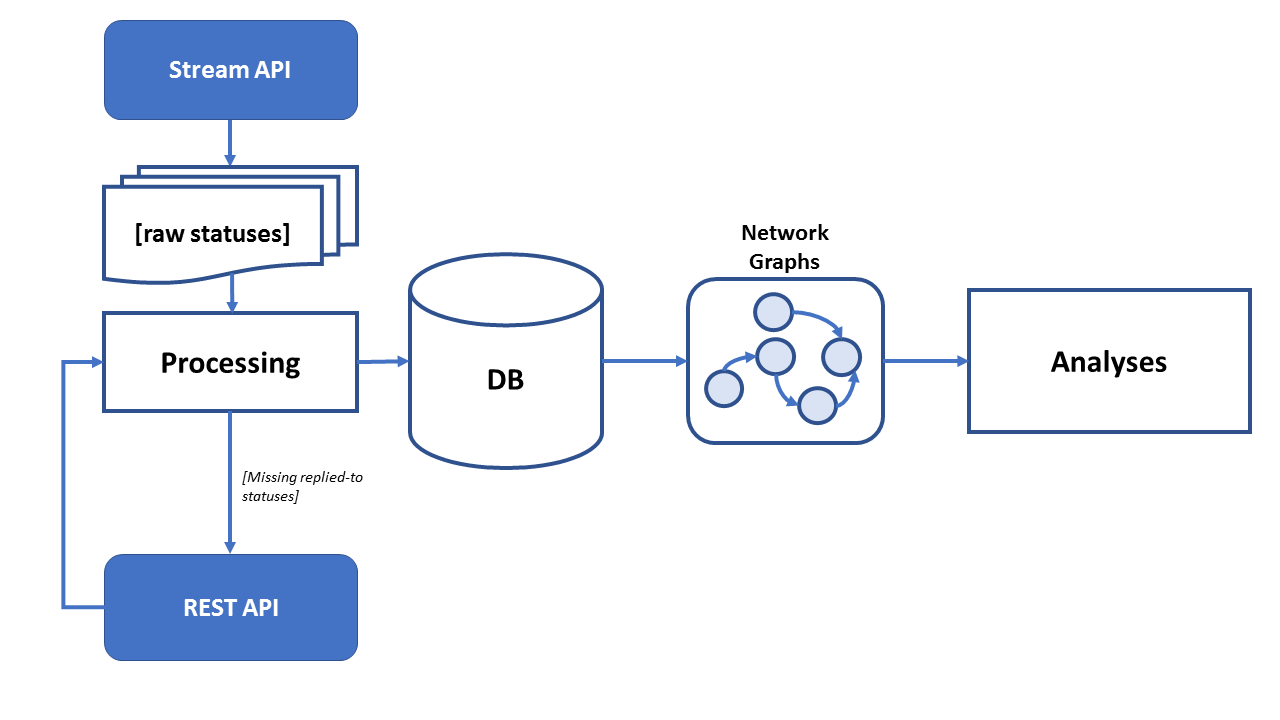
\includegraphics[width=\columnwidth]{images/frameworkstructure.png}
% \caption{Overall framework structure}
% \label{fig:frameworkstructure}
% \end{figure}

\subsection{Streaming}

To ensure we have as much data as possible, data collection takes
three steps. First, a stream endpoint is opened to catch activities of
accounts under investigation, those accounts will be referred to as
`watched' or `CS' (Customer Service) accounts. Twitter streaming API
is designed to return tweets created by the user, their retweets,
replies directed to their tweets, and retweets of their
tweets. However, the stream does not include tweets mentioning the
user, and replies/retweets by protected users. 

\subsection{Reply Chains}

Returned statuses from the Streaming API may represent reply to
statuses that have not been collected previously. It was found that most
missing statuses were either posted before data collection started, mentions, 
or the user account is protected. This issue could have a huge effect on 
analysis. 

Therefore, once statuses are returned from the stream endpoint, they
are processed to identify missing replied-to posts, and REST API is
used to collect them. This process runs recursively for newly
collected replies until no further replies are available. Unavailable
statuses are often result from either deletion or protected accounts.

Analysis of changes on the graph after the second phase of data
collection shows that there were increases in the number of nodes and
edges by 43\% and 62\%, respectively. This increase in connections has
resulted in merging 176 components into others, which improved
connectivity of the graph and, hence, accuracy of dependent analyses.

% \begin{figure}[htb]
% \centering
% 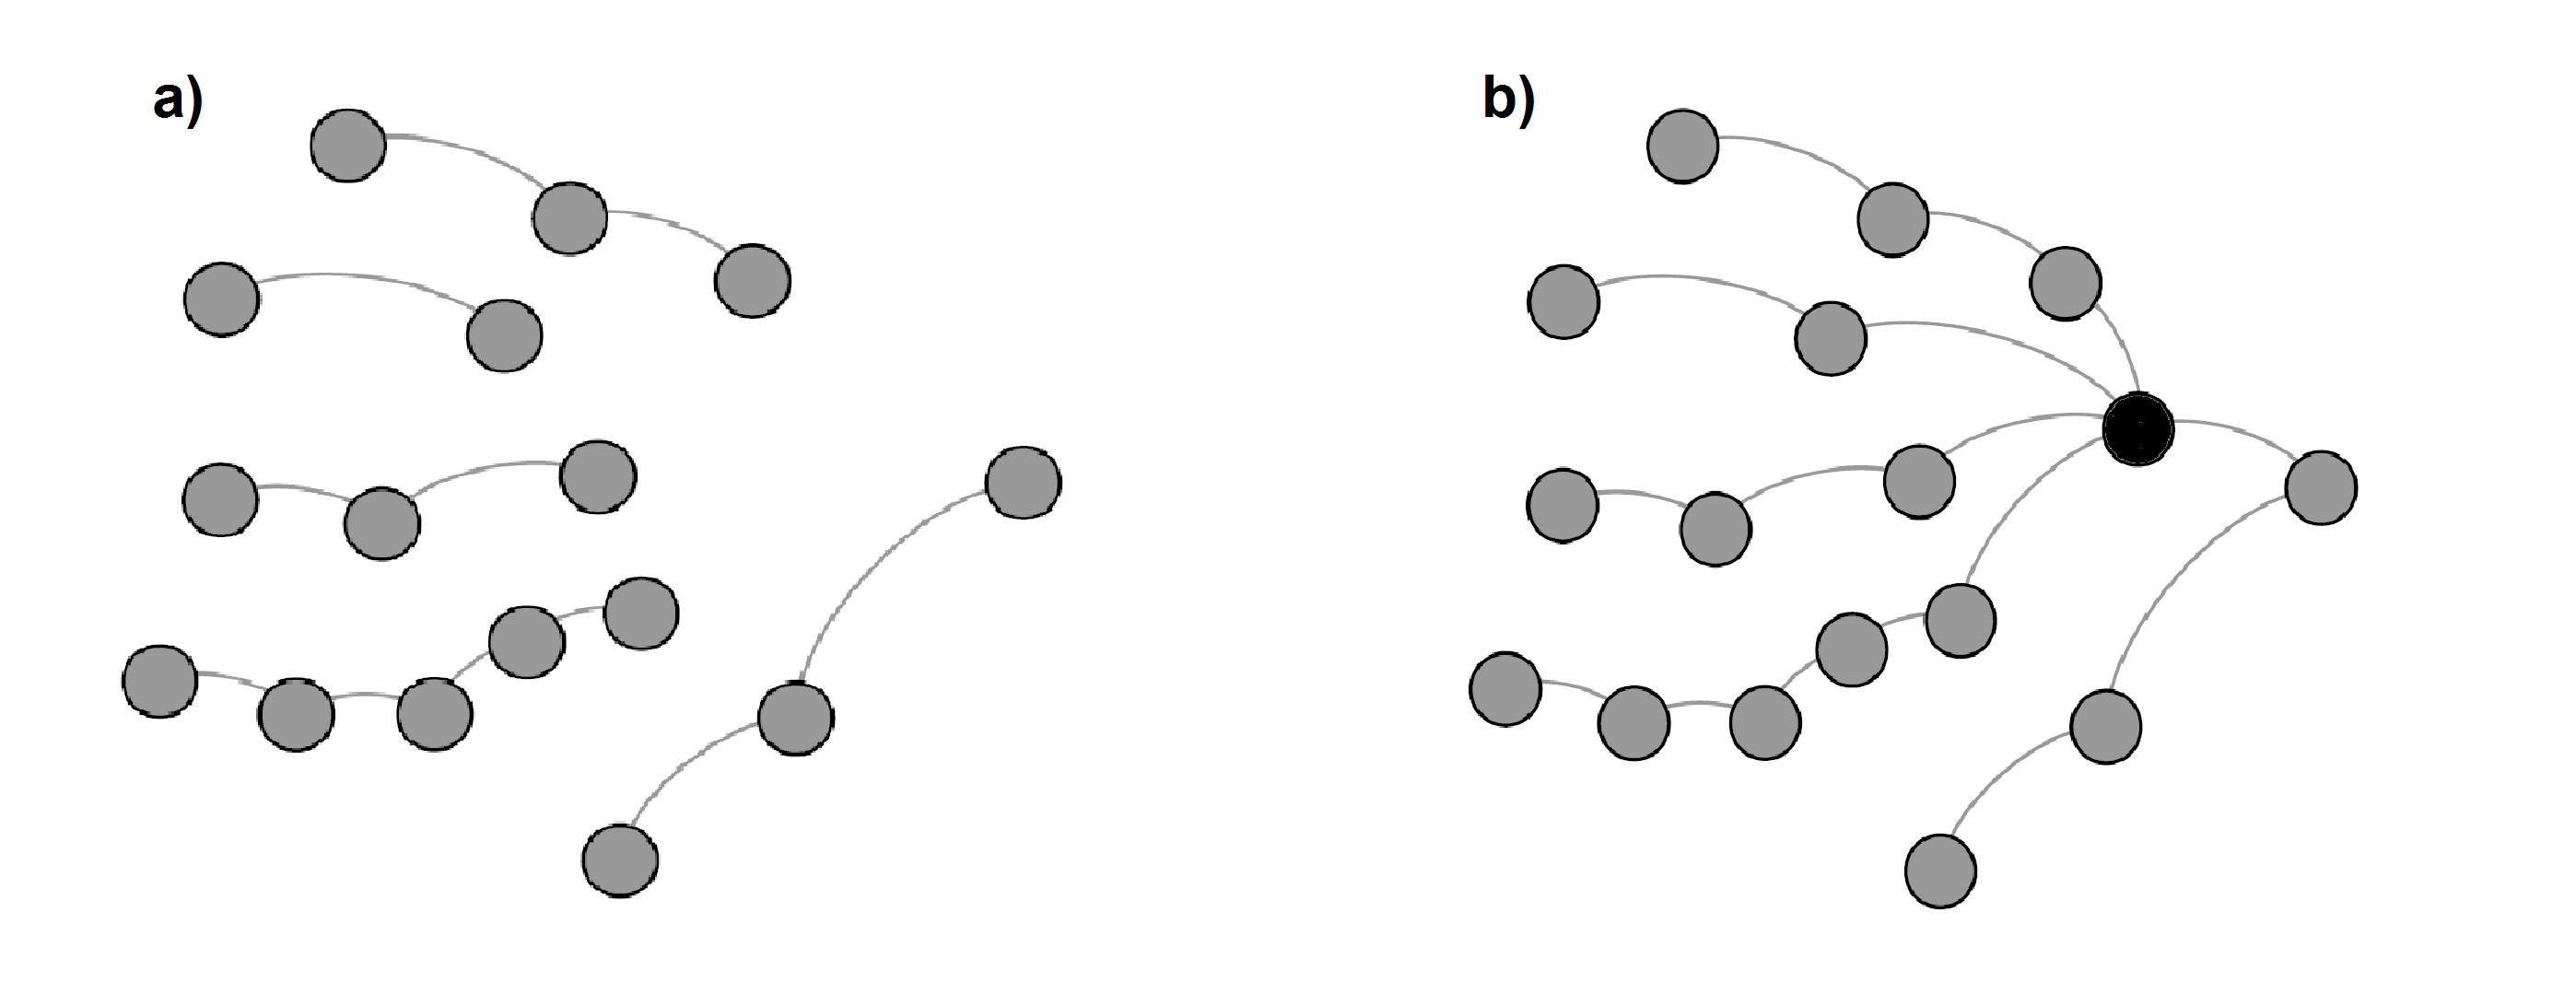
\includegraphics[width=\columnwidth]{images/datacollectionphases.png}
% \caption{(a) First phase of data collection and (b) second phase of data
% collection}
% \label{fig:datacollectionphases}
% \end{figure}


\subsection{Graph Construction}

\subsubsection{Main Graph}

Constructing graphs is the core of analyses presented in this work. 
First, a base graph\footnote{The terms `main graph' and `base graph' are 
used interchangeably.} is generated containing all replies and the needed data. 
Nodes represent post ids, while edges indicate replying direction. Other 
information of statuses are added as attributes to nodes. The information used in
this study are screen name of the user, timestamp of the reply, text,
and `watched' entity, to identify CS accounts. An example graph is
shown in Figure~\ref{fig:replychaingraph}. Properties of this graph
are constrained by how replies relate to each other. In other words,
no edge is expected to have weight value other than 1. Also, no reply
status can have outdegree greater than 1, however some nodes may have
an outdegree of 0. Node with outdegree=0 can be root nodes, i.e. first
post of conversation, or they were directed to unavailable
statuses. On the other hand, indegree of nodes can be 0 or
more. Special case nodes are those with indegree and outdegree equal
to 0. Those are isolated/floating nodes and must be removed before
analysis starts. First, those nodes do not benefit the analysis as
they are not part of any conversation. Second, they will be seen as
connected component by themselves, which affects accuracy of results.

\begin{figure}[htb]
\centering
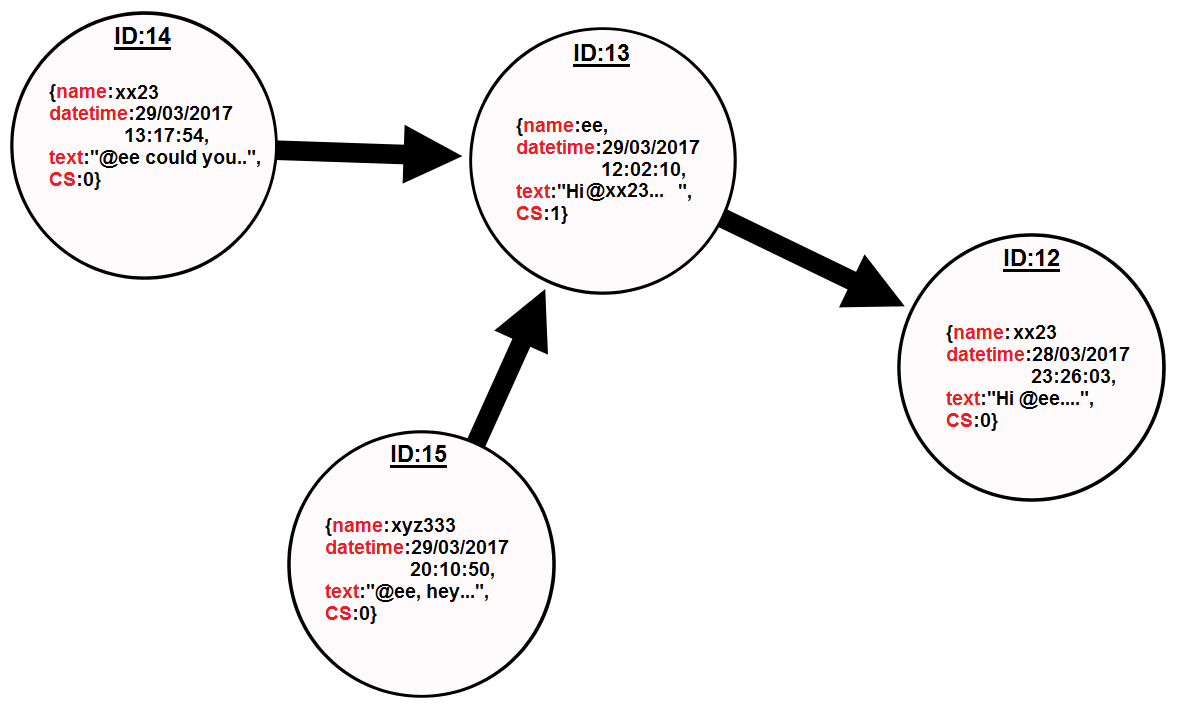
\includegraphics[width=\columnwidth]{images/replychaingraph.png}
\caption{Example of a reply chain graph}
\label{fig:replychaingraph}
\end{figure}

\subsubsection{Users' Graph}

Because most analyses focus on relationships between reply posts, they
were applied on the base graph. Nevertheless, to examine relationships
amongst users, another graph is generated from the base graph. This
process is carried out by iterating through edges linking reply posts,
extracting users' information, and constructing users graph
accordingly. In the context of this study, only two attributes are used, 
screen names and `watched' values. While nodes represent screen names 
`watched' valued are added as attribute of nodes. For edges, their weights 
indicate number of replies sent from origin node (sender) to target
node (receiver), therefore, the user graph is directed. Applying this
process on the example in Figure~\ref{fig:replychaingraph} results in
the users graph shown in Figure~\ref{fig:usersgraph}.

\begin{figure}[htb]
\centering
\includegraphics[width=\columnwidth]{images/usersgraph.png}
\caption{Example of users' graph extracted from base graph}
\label{fig:usersgraph}
\end{figure}

To examine relationships between users, five network graph properties
are measured. There were no special case nodes or edges in this graph,
as observed in the base graph. Graph properties that are used in
analysing this graph and their contextual interpretations are shown in
Table~\ref{tbl:uucentralitymeasuresinter}.

\begin{table}[!h]
\centering
\begin{tabularx}{\columnwidth}{lX}
\toprule
\textbf{Measure} & \textbf{Interpretation} \\ 
\midrule
{\emph{Indegree}} & Number of users that sent reply to the node \\
{\emph{Weighted Indegree}} & Total number of received replies \\
{\emph{Outdegree}} & Number of users that have received a reply from
                     the node \\ 
{\emph{Weighted Outdegree}} & Total number of sent replies \\
{\emph{Edge Weight}}& Number of replies between the connecting nodes\\
\bottomrule
\end{tabularx}
\caption{User-user centrality measures interpretation}
\label{tbl:uucentralitymeasuresinter}
\end{table}

\subsection{Connected Components}

The base graph consists of many number of subgraphs, each of which
represent related replies, i.e. one conversation entity. Investigating
connected components plays a major role in identifying conversations
for accounts. They are used to measure size of conversation, their
depths, and to identify shared conversations between watched
accounts. To extract conversations that user or users were engaged in,
the process iterates through nodes in each component and examine the
`name' attributes. As soon as the search is matched, no further nodes
are examined. Then, the component is either analysed on the fly, or
returned if more intensive analysis is required.

In the base graph, number of connected components reflect
conversations, while in users graph, connected components show users
communities. Therefore, in the base graph many components should be
expected, depending on activity of the watched accounts. However, in
the users graph, number of components should not exceed the number of
watched accounts, although there might be exactly one component due to
common customers.


\section{Results}\label{results}

\subsection{Accounts Activity}

Overall evaluation was carried to measure accounts activity. As shown in
Figure~\ref{fig:totalactivity}, {\emph{virginmedia}} was found the most 
active CS account by far. As the focus of this section is on customer services, 
it is necessary to investigate post types to examine purposes of
these accounts. The result shows that replies were at least 83.5\% of
accounts activity. This confirms that all chosen accounts are mainly
used to interact with customers and handling requests and
questions. Therefore, forthcoming analyses will be based on replies
only. 

\begin{figure}[htb]
\centering
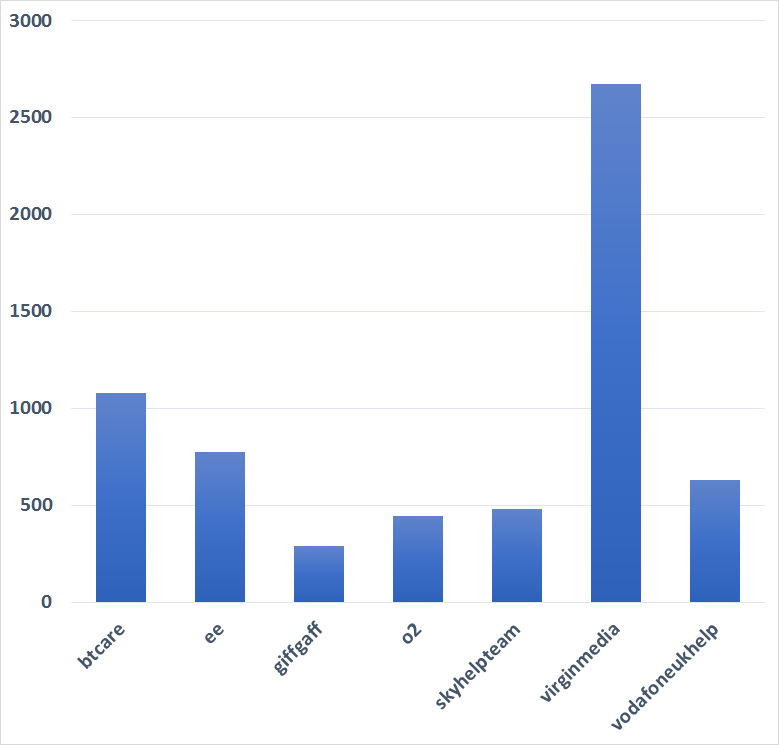
\includegraphics[width=\columnwidth]{images/totalactivity.png}
\caption{Total activity}
\label{fig:totalactivity}
\end{figure}

% \begin{figure}[htb]
% \centering
% 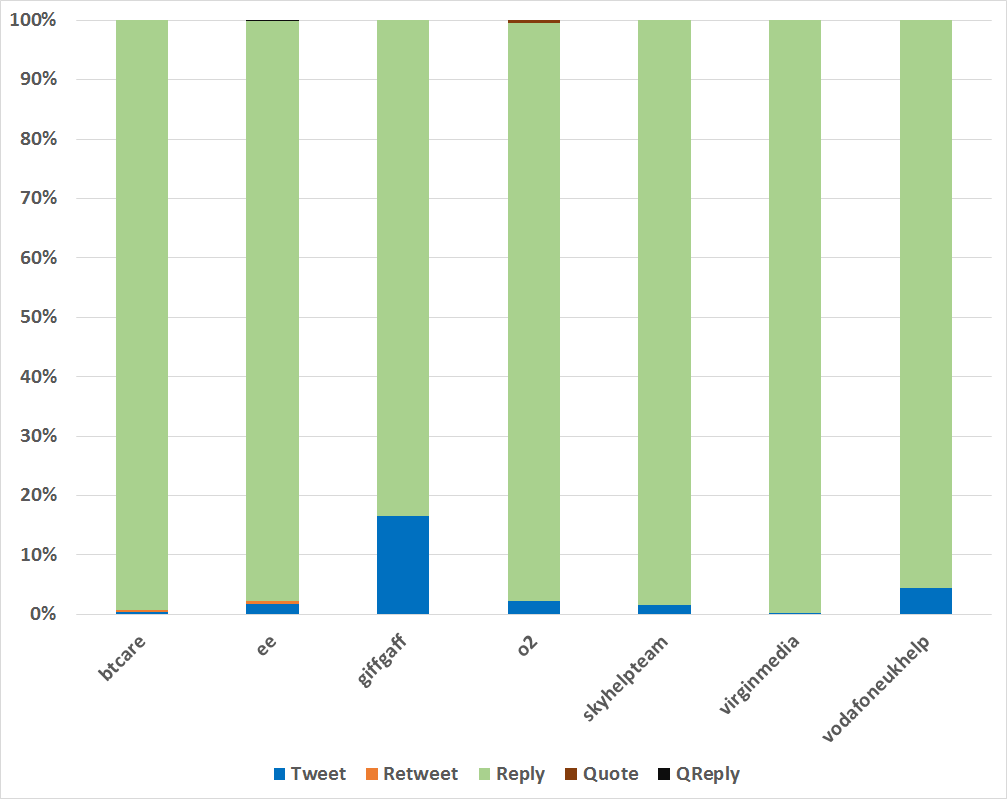
\includegraphics[width=\columnwidth]{images/accountsactivity.png}
% \caption{Accounts activity}
% \label{fig:accountsactivity}
% \end{figure}

\subsection{Interaction and Users}

Although working hours of CS accounts is important to evaluate
activity, it is important to measure posts that are directed to those
accounts from other users and examine them in line with CS
accounts. Audience and their relations with the accounts can be
analysed directly from the main graph (i.e. post-post). However, as
user details are embedded inside post nodes, observing such
relationships will not simple task to accomplish. Therefore, user-user
graph was built from the main graph. The resulted graph contains 3,521
user nodes and 5,938 edges, shown in
Figure~\ref{fig:userusergraph}. Although post-post relationship cannot
have weight higher than one, user-user edge weight indicates number of
posts in one direction, which explains the reduction in number of
nodes and edges.

\begin{figure}[htb]
\centering
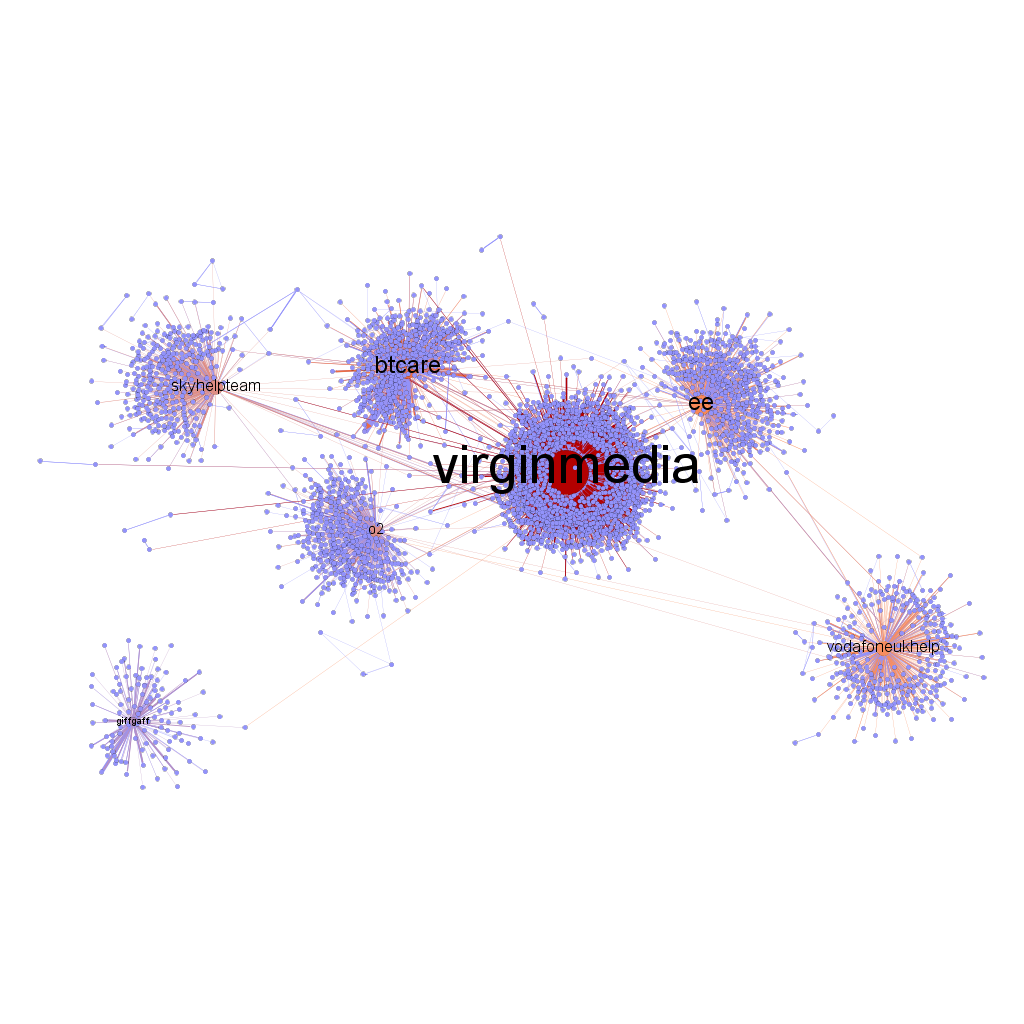
\includegraphics[width=\columnwidth]{images/userusergraph.png}
\caption{User-user graph}
\label{fig:userusergraph}
\end{figure}

Based on Table~\ref{tbl:uucentralitymeasuresinter}, summary of the
graph is presented below in Table~\ref{tbl:uucentralitymeasures}. The
table says that {\emph{virginmedia}} received that highest number of
replies from 866 users with an average of 3.05 per user. Also, the
same account scored highest in number of recipients. The difference
between indegrees and outdegrees shows that apart from {\emph{o2}},
all accounts have outdegrees bigger that their
indegrees. Additionally, total number of sent replies is found to be
more than the number of received replies. This may reflect that those
replies were directed to non-reply posts.

\begin{table}[!h]
\centering
\begin{tabularx}{\columnwidth}{l|rrc|rrc}
\toprule
\textbf{Measure} & \textbf{ind} & \textbf{w.ind} & \textbf{\%} & \textbf{out} & \textbf{w.oud} & \textbf{\%}\\ 
\midrule
{\emph{btcare}} & 330 & 995 & 3.02 & 485 & 1317 & 2.72\\
{\emph{ee}} & 247 & 432 & 1.75 & 470 & 778 & 1.66 \\
{\emph{giffgagg}} & 77 & 209 & 2.71 & 102 & 247 & 2.42 \\ 
{\emph{o2}} & 293 & 463 & 1.58 & 260 & 479 & 1.84 \\
{\emph{skyhelpteam}} & 147 & 254 & 1.73 & 305 & 504 & 1.65\\
{\emph{virginmedia}} & 866 & 2645 & 3.05 & 1215 & 3421 & 2.82\\
{\emph{vodaphoneukhelp}} & 166 & 403 & 2.43 & 302 & 660 & 2.19\\
\bottomrule
\end{tabularx}
\caption{Centrality measures of user-user graph}
\label{tbl:uucentralitymeasures}
\end{table}

\subsection{Delay}\label{results_delay}

Observation of active hours provides an overall view of
account activity. However, calculating delays is important to provide
more insights on performance of CS team. As reply nodes in the base graph (post-post)
include timestamp attribute, measuring delay was acheived by calcuating temporal
differences between end nodes on each edge. Table~\ref{tbl:delaystats} 
shows descriptive statistics for CS account delays. Interestingly, 
{\emph{skyhelpteam}} was found with an average delay of 45.04 hours,
although rest of the CS accounts' delay ranged between 1.14 and 3.34 hours. 

% \begin{figure}[htb]
% \centering
% 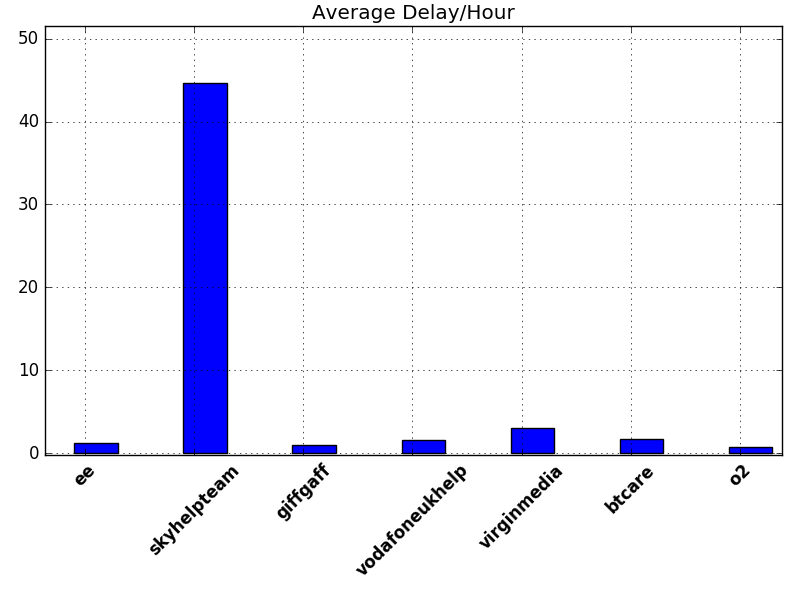
\includegraphics[width=\columnwidth]{images/delaymeans.png}
% \caption{Delay means for CS accounts}
% \label{fig:delaymeans}
% \end{figure}

\begin{table}[!h]
\centering
\begin{tabularx}{\columnwidth}{lrrrr}
\toprule
\textbf{Account} & \textbf{mean} & \textbf{stdev} & \textbf{max} & \textbf{min(sec)} \\ 
\midrule
{\emph{btcare}} & 2.04 & 16.11 & 572.46 & 38\\
{\emph{ee}} & 1.46 & 3.39 & 19.28 & 27\\
{\emph{giffgagg}} & 1.22 & 10.25 & 159.97 & 73\\ 
{\emph{o2}} & 1.14 & 2.66 & 22.48 & 58\\
{\emph{skyhelpteam}} & 45.04 & 49.16 & 117.21 & 44\\
{\emph{virginmedia}} & 3.34 & 9.25 & 263.98 & 22\\
{\emph{vodaphoneukhelp}} & 1.92 & 5.01 & 76.51 & 50\\
\bottomrule
\end{tabularx}
\caption{Summary delays statistics}
\label{tbl:delaystats}
\end{table}

\subsection{Conversation Components}

As covered in the mehtodology, each connected component in the post-post 
graph represent a conversation entity that includes related replies. 
In this dataset, there were 3,289 conversation components with various number
of replies. Observsation of their sizes shows that the smallest component
consists of one post, while the biggest component contains 81 posts. 
Furthermore, the number of one-post components was 102, and they were all 
found belonging to CS accounts. Examining those singular components revealed that 
they were either original tweets that have no replies or replies with no
replied-to post available. As covered earlier, missing replies are those that 
could not be captured due to a deletion or their posting account was protected. 
Because they do not have any length, and hence do not represent an examinable
conversation, single-node components will be excluded from forthcoming
analyses.

Additionally, most common size of connected components was found to be two nodes. 
They were 1,188 components and the direction of their edges revealed
that most of these communications were from CS accounts and directed
to customer's post. However, 25 of those conversations were initiated by customers. 
As they are in two-node components, this shows that those posts have not been 
answered by CS. Although other means of communications could have been used, such as 
direct messages, there were no visible sign of such interaction.

% \begin{figure}[htb]
% \centering
% 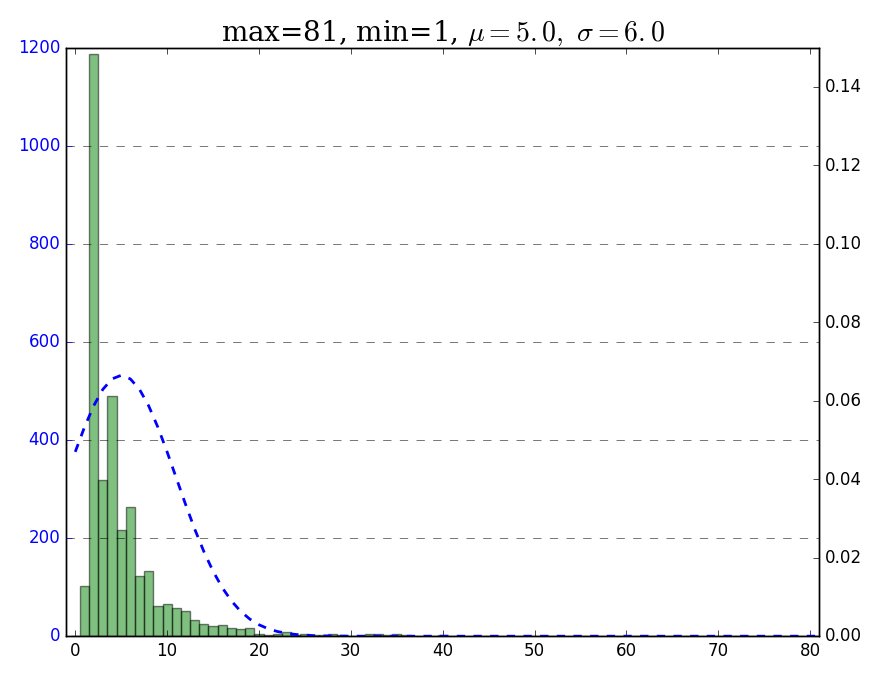
\includegraphics[width=\columnwidth]{images/ccsizes.png}
% \caption{Connected component sizes}
% \label{fig:ccsizes}
% \end{figure}

\subsection{Component Size and Longest Path}

It is important to note that the size of connected components does not
necessarily reflect length of conversations, although there is a
strong correlation between size of component and length of its longest
path (0.88). As can be seen in Figure~\ref{fig:ccsizepaths}, many components
measures are positioned near perfect diagonal line. Interestingly, the 
longest path in the biggest component (81 nodes/posts) was only 1.

\begin{figure}[htb]
\centering
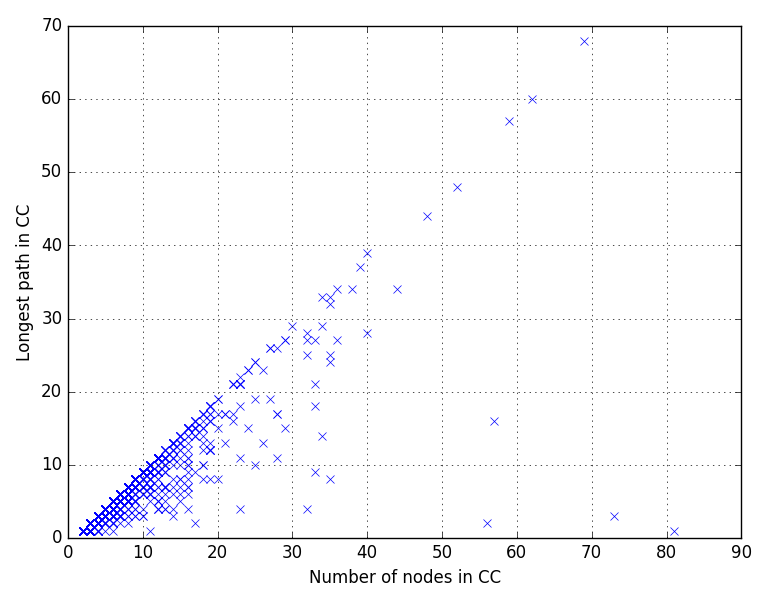
\includegraphics[width=\columnwidth]{images/ccsizepaths.png}
\caption{Size of components and their longest paths}
\label{fig:ccsizepaths}
\end{figure}

To further explore properties of connected components, biggest 20
components, shown in Figure~\ref{fig:20ccpostpostgraph}, were examined. 
The findings show that components with very high variations in indegree
amongst their nodes are mostly originate from CS. Examples of this claim 
is illustrated by the three big components in the figure. When observed, they 
were found featuring tweets of advert. Another observation on the biggest 
component is that origin node was a post by {\emph{o2}} and 
has an indegree of 80, while rest of the nodes have indegree of zero, i.e. they 
were not answered. On the other hand, the longest path component was ranked the 
third biggest component. It was found with a single leaf, and all other nodes along
the path were found with indegree=1 and outdegree=1, forming what we call {\emph{simple
chain}}, uniquely coloured in Figure~\ref{fig:20ccpostpostgraph}. Additionally, 15 of those
components were found to have originated from customer accounts, and
they all take a semi-simple chain.

\begin{figure}[htb]
\centering
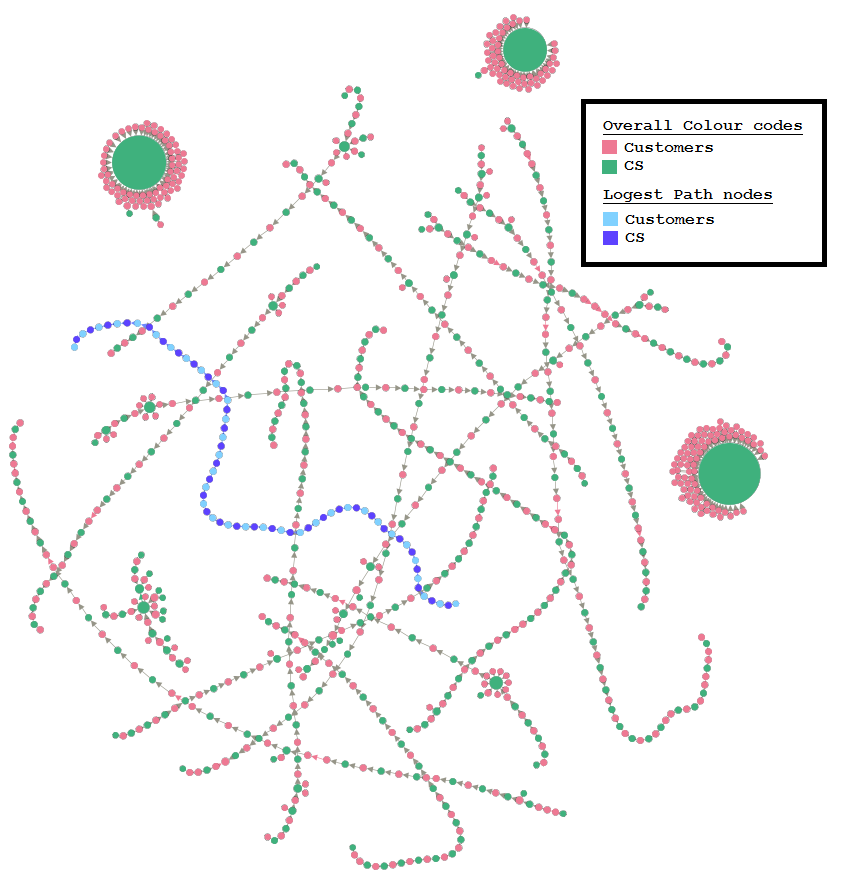
\includegraphics[width=\columnwidth]{images/20ccpostpostgraph.png}
\caption{Largest 20 connected components in post-post graph}
\label{fig:20ccpostpostgraph}
\end{figure}

Generally, simple chains can be identified where number of edges
equals length of the longest path in component. Simple chains account for 80\%
of the connected components in graph, of which 47\% were found 
with the length of 1. This is in alignment with the
results of connected component sizes presented earlier. Finally,
Table~\ref{tbl:delaystatscl} presents statistics on chains of
individual CS accounts.

% \begin{figure}[htb]
% \centering
% 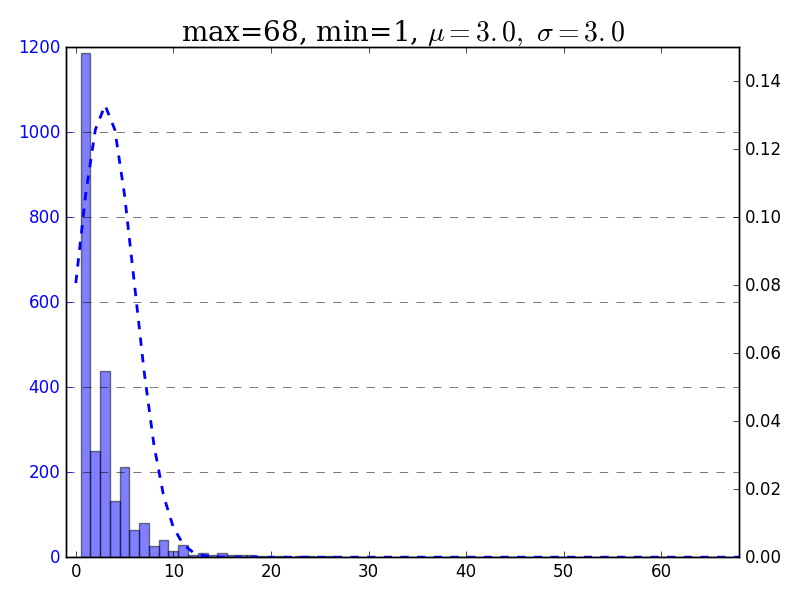
\includegraphics[width=\columnwidth]{images/simplechainlengths.png}
% \caption{Simple chain lengths}
% \label{fig:simplechainlengths}
% \end{figure}

\begin{table}[!h]
\centering
\begin{tabularx}{\columnwidth}{lrrrrr}
\toprule
\textbf{Name} & \textbf{count} & \textbf{max} & \textbf{min} & \textbf{mean} & \textbf{stdev}\\ 
\midrule
{\emph{btcare}} & 388 & 19 & 1 & 3.46 & 3.22\\
{\emph{ee}} & 324 & 9 & 1 & 1.98 & 1.43\\
{\emph{giffgagg}} & 147 & 12 & 1 & 2.39 & 1.98\\ 
{\emph{o2}} & 216 & 11 & 1 & 2.53 & 2.26\\
{\emph{skyhelpteam}} & 252 & 15 & 1 & 2.22 & 1.99\\
{\emph{virginmedia}} & 959 & 68 & 1 & 3.78 & 4.46\\
{\emph{vodaphoneukhelp}} & 248 & 39 & 1 & 2.58 & 3.29\\
\bottomrule
\end{tabularx}
\caption{Summary statistics on chain length for CS accounts}
\label{tbl:delaystatscl}
\end{table}

\subsection{Coexistence and Competition}

Connected components were utilised to investigate competition amongst 
CS accounts. This was achieved by first identifying components that include 
more than one CS account. For each connected component, notes are 
checked in turn to examine their names. Components with more than one name
are then marked as coexistence component. The results show that there were 
39 common components, 38 have two CS accounts, and one includes three 
accounts. The graph presented in Figure~\ref{fig:commoncc} shows those 
components, with each CS account given a colour code for identification as 
the legend clarifies.

\begin{figure*}[htb]
\centering
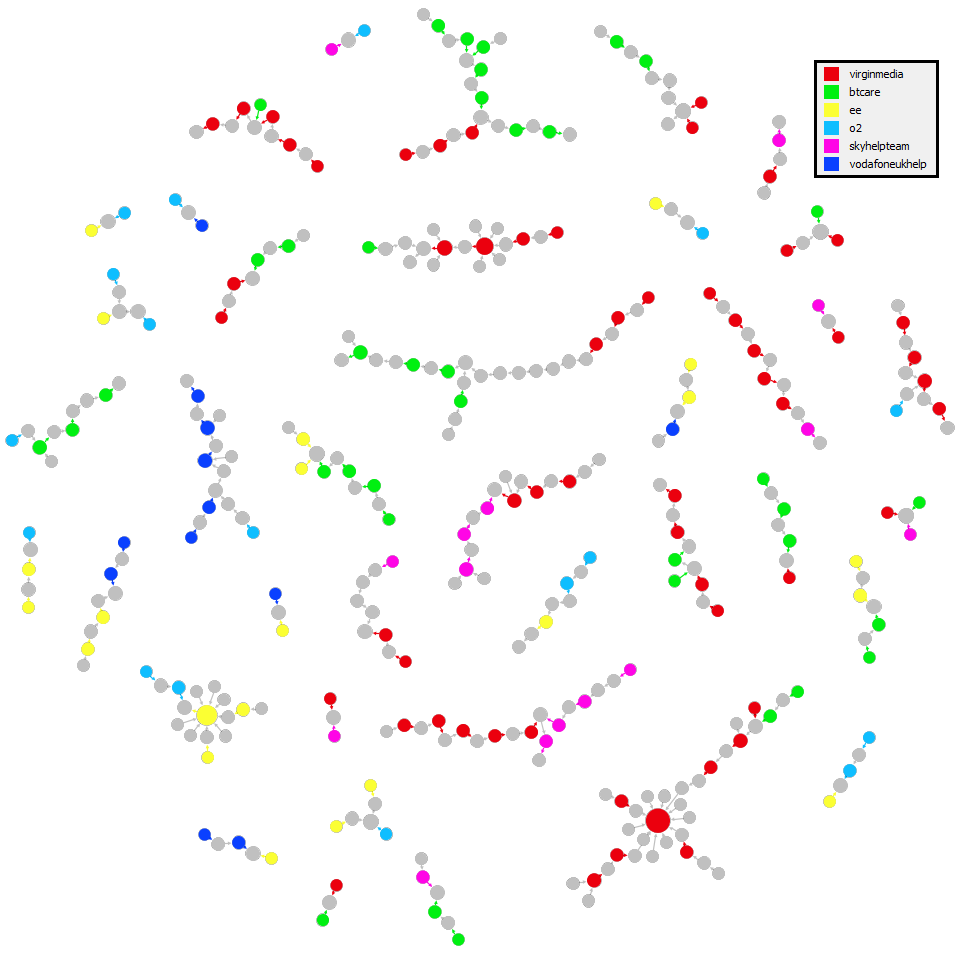
\includegraphics[width=0.6\textwidth]{images/commoncc.png}
\caption{Common connected components}
\label{fig:commoncc}
\end{figure*}

To explore these relationships further, a specific users graph was constructed 
based on those components. Construction of this graph follows similar steps used in 
customer-CS graph. However, as CS accounts do not have direct engagement 
with each other, edges in this graph are undirected and their weights indicate number 
of times they appeared together in the same conversation component. 
The resulted CS-CS graph is shown in Figure~\ref{fig:coexistencegraph}, where 
node size indicates degree of node to show how many other CS accounts the node 
has coexisted with, while darkness of node reflects weighted degree to show the 
total frequency of coexistence for the node.   

First observation on the graph is that {\emph{giffgaff}} account was not found in 
any common conversation. In contrast, {\emph{o2}} was the only account
that have shared conversations with all other CS accounts, while
{\emph{vodafoneukhelp}} was found with least common
conversations. Nevertheless, weighted degree measure shows that
{\emph{virginmedia}} was the highest in number of common
conversations, 21 components, although its degree tells that those 
conversations were shared with only 3 other CS teams. The heaviest edge
existed between {\emph{virginmedia}} and {\emph{btcare}}, followed by
the edge between {\emph{virginmedia}} and {\emph{skyhelpteam}}. Also,
edges of {\emph{o2}} show that it was mostly appeared with
{\emph{ee}}, and for {\emph{vodafoneukhelp}} it was {\emph{ee}}.

The observation of edges and their weights can provide insights to
uncover more specific service areas within the business domain. This
was found clear when modularity of the graph was examined. The result
has unfolded into two communities, as shown in
Figure~\ref{fig:modularityclassgraph}. Also, general knowledge about
those CS teams; {\emph{ee}}, {\emph{o2}}, and {\emph{vodafoneukhelp}}
belong to business domain that is mostly focused on mobile services,
while {\emph{skyhelpteam}}, {\emph{virginmedia}}, and {\emph{btcare}}
are mostly known to be focusing on home internet and landline
services.

\begin{figure}[htb]
\centering
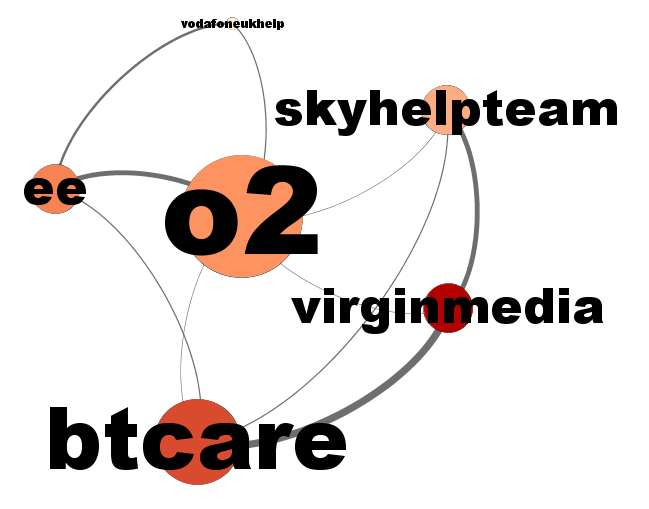
\includegraphics[width=\columnwidth]{images/coexistencegraph.png}
\caption{CS-CS coexistence graph}
\label{fig:coexistencegraph}
\end{figure}

\begin{figure}[htb]
\centering
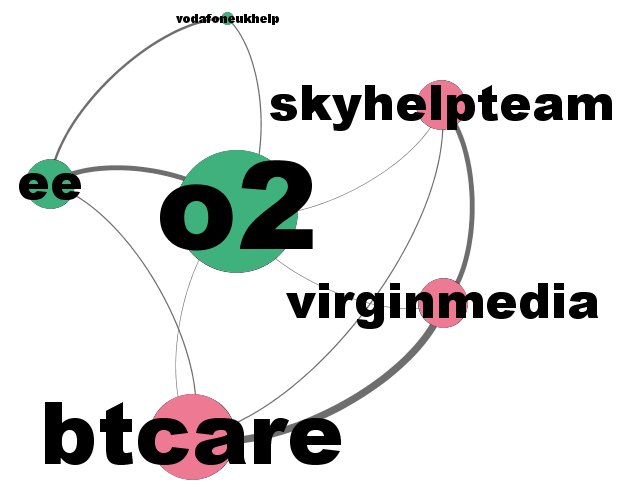
\includegraphics[width=\columnwidth]{images/modularityclassgraph.png}
\caption{Modularity class graph}
\label{fig:modularityclassgraph}
\end{figure}

Furthermore, using similar approach that was used in \ref{results_delay}, 
delay was measured in those components to evaluate if presence of competitor 
has influence on how quick CS team response. Interestingly, improvement of
26\%, 43\% and 72\% were observed for {\emph{virginmedia}},{\emph{btcare}}
and {\emph{skyhelpteam}}, respectively. Rather strangely, for the other 
three companies, the average delay showed a drop by at least 9\%.

% \begin{figure}[htb]
% \centering
% 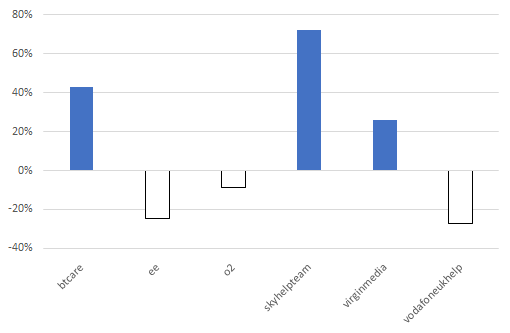
\includegraphics[width=\columnwidth]{images/diffdelaymeans.png}
% \caption{Modularity class graph}
% \label{fig:diffdelaymeans}
% \end{figure}

% To better understand the context of conversations in those common
% components, text analysis was carried out for each CS account. The
% attempt is a try to find what the customer have said that made the CS
% team participate in the conversation. Therefore, posts of CS accounts
% were eliminated, and the analysed texts include posts of customers
% only. Presentation of the result could be shown in table of statics,
% rather, wordcloud visualisation was used for each CS account. Initial
% results show that mentions were found very high in number. Therefore,
% another one was generated after removing mentions, results are
% presented in Figure ‎2.17.

% Interestingly, the first set of results (with mentions) provide
% explanation and insights on edge weights shown in
% Figure~\ref{fig:20ccpostpostgraph}. Taking one example, the edge
% {\emph{virginmedia}}--{\emph{btcare}} was found the heaviest. However,
% the first set of wordclouds for both show that {\emph{virginmedia}}
% was the mostly mentioned by customers. Same conclusion was found for
% the edge {\emph{skyhelpteam}}--{\emph{virginmedia}}.

% The other set, with mentions removed, may be used to identify some
% keywords for what could possibly be main issues, problem, or complains
% that might be of advantageous to other business rivals.


\section{Discussion}\label{discussion}

The analysis of selected CS accounts started with measuring statuses
type to testify whether the CS account are dedicated for customer
services or not. This step is important to confirm that accounts are
similar in their purposes, hence comparison would be fair and valid.

Volume of account activity and served customers and their interactions
with the account give measures on popularity of the account on Twitter
and may help make inferences on the size of their customers who are on
Twitter. From these three measures, {\emph{virginmedia}} was found with
highest volume of posts, the least diverse in terms of type of posts
(99.7\% were replies) and has the highest number of customers.

The results also show that high availability, i.e. longer activity
hours, was not found to significantly improve speed of reply to
customers. Also, average delays of accounts ranged between 1.14 and
3.34 hours, apart from {\emph{skyhelpteam}} which was found with an average
delay of 45.04 hours. This may indicate a management issue for the
team, such as unclear social media strategy and team size. 

In the analysis of common/shared connected components, competition was
found to have taken place amongst accounts. Particularly, in the case
of {\emph{virginmedia}} and {\emph{btcare}} the competition was
obvious and severe. Although no record shows that CS team has been in
a direct engagement with a competitor, the conversations were directed
to customers. In all cases, customers were found to be initiators of
competing conversations by making use of Twitter mention feature to
bring different rivals into conversations. In contrast to phone or
email, complaints that are taken to social media are perceived as more
damaging to the business reputation. Therefore, improvement in the
speed of response was witnessed in few cases where business rivals
appeared in the same conversation. This indicates that the platform
helps customers tend to take the advantage of Twitter to win good
deals or speed resolving their problems. Additionally, although all
accounts were from telecommunication domain, competition analysis
uncovered more specialised communities.


\section{Conclusions}\label{conclusions}

The paper has presented a framework for evaluating customer services
performance and their communities on Twitter. Network graphs
properties lay in core of all analyses to obtain the presented
results, and were applied on some selected accounts in the telecoms
business domain in the UK.

As shown in the Section~\ref{method}, there are two preliminary
techniques that need to be applied prior to starting the analysis
phase. First, the recursive reply-chain data collection is a crucial
stage in obtaining more accurate results. The importance of this stage
stems from the fact that it fills the gaps and improve connectivity of
graphs. Second, construction of the initial graph from replies and the
removal of floating isolated nodes. Then, it is a matter of correctly
choose needed information and attach them as attributes to nodes. In
this study, information included were id of post, timestamps, screen
name, text and watched flag. Nevertheless, the framework can be
extended to include other information such retweets.

Furthermore, once the main graph is constructed, other graphs could be
generated based on purposes of analysis. The connected components
section showed how conversations of certain features can be extracted
for further analysis. Examples presented in the section include
lengths of conversations and coexistence of business rivals.

The presented framework can be used by service providers to evaluate
their social media accounts, as well as make observations about their
rivals within the domain. Moreover, with the emerging practice of
signing reply with member initials, this practice can be exploited to
extend this framework. This extension could help in estimating team
sizes, working shifts and to evaluate individual team members. Another
application would be to identify gaps, competitions, challenges and
opportunities in services that can be used in drawing strategies for
start-ups for example. The approach can also be applied to other
domains or contexts, such non-profit or government institutes. Also,
it can be used for group of users, such as celebrities and their
direct and indirect confrontations on Twitter.

% \section*{Acknowledgements}

% This work has been supported by a doctoral research scholarship for
% Nabeel Albishry from King Abdulaziz University, Kingdom of Saudi
% Arabia.


\bibliographystyle{ACM-Reference-Format}
\bibliography{ssei2018} 

\end{document}
